\documentclass[12pt,a4paper,titlepage]{article}
\usepackage[utf8]{inputenc}
\usepackage[finnish]{babel}
\usepackage{setspace}
\usepackage{parskip}
\usepackage{amssymb}
\usepackage{amsmath}
\usepackage{graphicx}
\usepackage{fancyhdr}
\usepackage[top=1in, bottom=1in, left=1in, right=1in]{geometry}
\usepackage{float}
\usepackage[section]{placeins}
\usepackage{listings}
\usepackage{courier}
\usepackage{subcaption}
\usepackage{textcomp}
%\usepackage[numbered,autolinebreaks,useliterate]{mcode} % jos tahdot laittaa matlabkoodia näkyville niin kannattaa käyttää tätä

% hyödyllisiä paketteja:
\usepackage{siunitx}\sisetup{per=frac} % SI-yksiköitä.
%\usepackage{supertabular} % jos tarttee isoja taulukoita
%\usepackage{fullpage} % pienemmät marginaalit jos haluaa

\lstset{basicstyle=\ttfamily,breaklines=true}

\usepackage{hyperref} % lisääthän omat pakettisi ENNEN hyperref'iä
\hypersetup{pdfborder={0 0 0}}
\onehalfspacing
\cfoot{}
\rhead{\thepage}
% asettaa nyk. kappaleen nimen vasempaan ylänurkkaan, saa poistaa jos haluaa
\lhead{\leftmark}

%%%%% kaikki ennen tätä liittyy käytettäviin paketteihin tai dokumentin muotoiluun. siihen ei tarvinne aluksi koskea. %%%%%

%%%%% kansilehti %%%%%
\title{Advanced Dynamics \\ The Plutonian Course Project \vspace{0.5em}}
\author{Anni Järvenpää}
\date{\today}
\begin{document}
\maketitle

% Sisällysluettelo
%\newpage
%\thispagestyle{empty}
%\tableofcontents
%\newpage
%\setcounter{page}{1}
%\parskip=1em \advance\parskip by 0pt plus 2pt
%\pagestyle{fancy}

% prosenttimerkillä alkavat rivit ovat kommentteja: niitä ei katsota dokumenttia käännettäessä eli ne ovat vain kirjoittajaa varten

%%%%%%%%%%%%%%% Oleellinen sisältö alkaa%%%%%%%%%%%%%%%

\section{Integraattorit}
Valitsin toteutettaviksi integraattoreiksi leapfrog-integraattorin ja neljännen asteen Runge-Kutta -integraattorin. Kummankin lähdekoodi löytyy GitHub-repositoriosta \url{https://github.com/aajarven/AD-integrators} löytyvästä \texttt{\href{https://github.com/aajarven/AD-integrators/blob/master/integrators.c}{integrators.c}}-tiedostosta. Repositorio sisältää myös muut ohjelman suorittamiseen tarvittavat tiedostot makefilen, joka luo ajettavan binäärin polkuun \texttt{bin/main}. Tämän jälkeen ohjelma on mahdollista ajaa komennolla
\begin{lstlisting}
./bin/main input nBodies dimensions step end outFreq output integrator
\end{lstlisting}
missä \texttt{input} on polku alkuehtoihin, \texttt{nBodies} kertoo simulaation kappaleiden määrän, \texttt{dimensions} käytettyjen ulottuvuuksien määrän, \texttt{step} on aika-askelen pituus päivissä, \texttt{end} on simulaation pituus päivissä, \texttt{outFreq} määrää kuinka monen aika-askelen välein tilanne kirjoitetaan tiedostoon ja \texttt{integrator} on joko \texttt{l} tai \texttt{r} jolloin käytetään integraattorina joko leapfrogia tai Runge-Kuttaa. Liian pieni määrä parametreja johtaa virheilmoituksen näyttämiseen ja ohjelman suorituksen päättymiseen, virheelliset parametrit puolestaan johtavat ohjelman kaatumiseen määrittelemättömällä tavalla tai virheellisiin tuloksiin.

Input-tiedoston tulee sisältää kunkin kappaleen koordinaatit, nopeudet ja massat tässä järjestyksessä välilyönnein eroteltuna omilla riveillään. Kommenttimerkkinä toimii \texttt{asdf}, jolla alkavia rivejä ei käsitellä. Samoin tyhjät rivit jätetään huomiotta.

Kumpikin integraattori vaikuttaa toimivan ja tuottaa järkeviä ratoja. Kuvassa \ref{lf-vuosi} on esitetty ulkoplaneettojen ja Auringon paikat noin yhtä Pluton radan etäisyydellä tehtyä ratakierrosta vastaavan 250 vuoden ajanjakson aikana integroituna leapfrog-integraattorilla ja vastaavasti kuvassa \ref{rk-vuosi} on käytetty RK4-integraattoria. Ennen kunkin outputin kirjoittamista tiedostoon kappaleiden massakeskipiste siirretään koordinaatiston origoon, jolloin Aurinko pysyy aina likimain origossa.

Integraattorin outputit sisältävät sarakkeittain kunkin kappaleen indeksin, tallennushetken, koordinaatit ja nopeudet. Kappaleet on indeksoitu nollasta alkaen siten, että järjestys on sama kuin input-tiedostossa. Yksikköinä on ajoille päivä, koordinaateille AU ja nopeuksille AU/d.

Riittävän lyhyttä aika-askelta käytettäessä kummankin integraattorin antamat tulokset vastasivat hyvin toisiaan, kuten seuraavissa luvuissa näytetään. Suorituskyvyltään RK4 on jonkin verran huonompi. Osittain tämä johtuu menetelmän luonteesta, mutta jonkin verran vaikuttaa todennäköisesti oma toteutukseni, jossa esimerkiksi kunkin aika-askeleen aikana luodaan ja vapautetaan useita kookkaita taulukoita k-kertoimien laskennassa tarvittavien väliaikaisten paikkojen ja nopeuksien tallentamiseen.

\begin{figure}
\centering
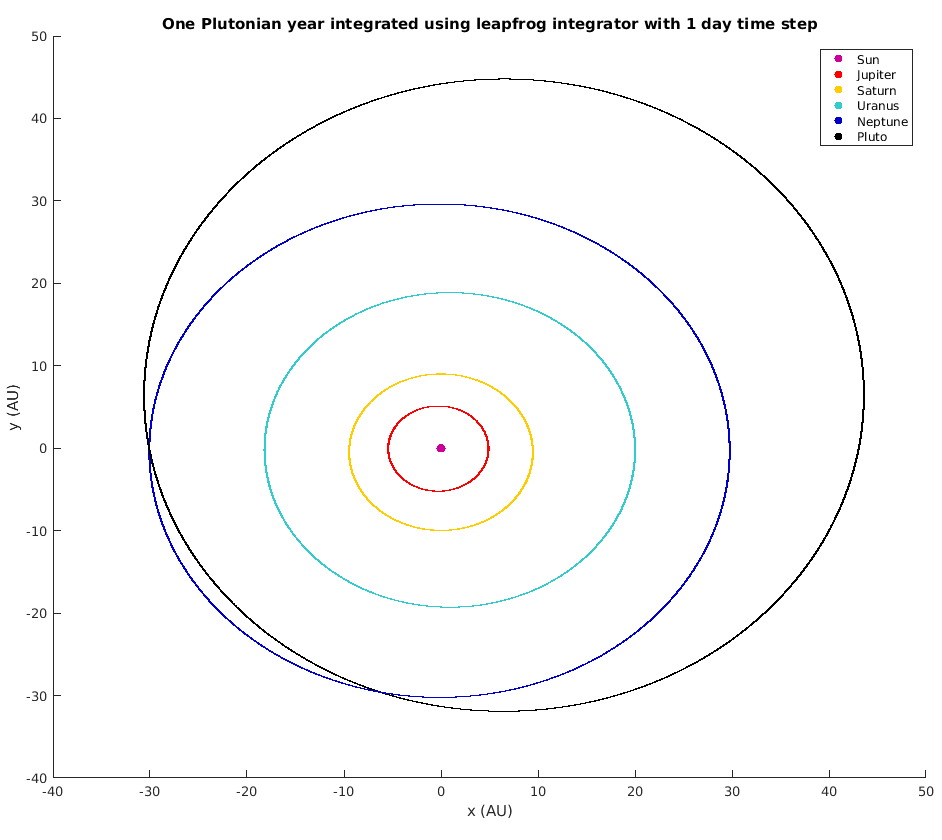
\includegraphics[width=\textwidth]{../plots/vuosi-leapfrog-cut.png}
\caption{Ulkoplaneettojen radat 250 vuoden ajanjakson aikana leapfrogilla integroituna. Aurinkoa edustava merkki on muita suurempi, jotta se erottuu, vaikka sen liike on hyvin vähäistä.}
\label{lf-vuosi}
\end{figure}

\begin{figure}
\centering
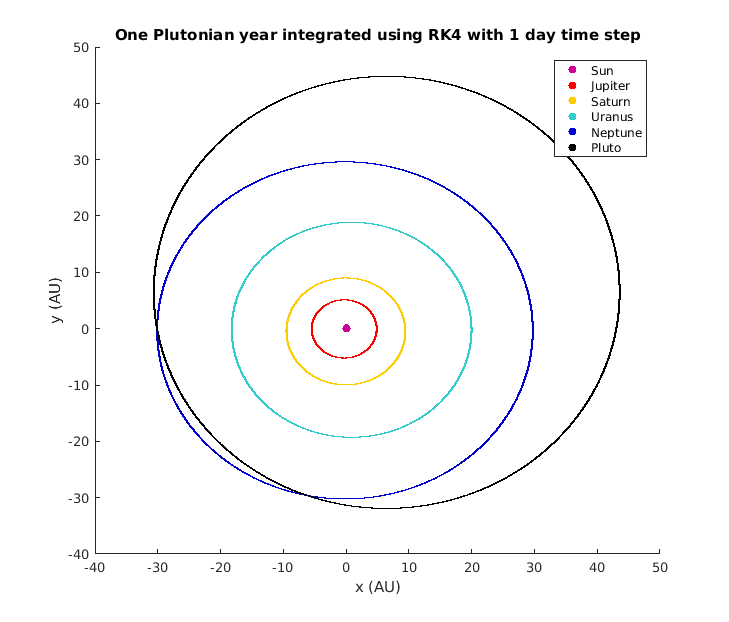
\includegraphics[width=\textwidth]{../plots/vuosi-rk4.png}
\caption{Ulkoplaneettojen radat 250 vuoden ajanjakson aikana RK4-integraattorilla integroituna. Aurinkoa edustava merkki on muita suurempi, jotta se erottuu, vaikka sen liike on hyvin vähäistä.}
\label{rk-vuosi}
\end{figure}


\section{Rataelementit}
Rataelementtien laskemisen toteutin Matlabilla. Tähän tarkoitukseen luotu funktio\\\texttt{\href{https://github.com/aajarven/AD-integrators/blob/master/plottaus/planetElements.m}{planetElements(planetNumber, mu, x, y, z, vx, vy, vz, t, index)}} laskee annetun indeksin omaavan planeetan inklinaation $i$, keskianomalian $M$, perihelin argumentin $\omega$, nousevan solmun pituuden $\Omega$, eksentrisyyden $e$, näitä vastaavat ajanhetket sekä parametrin 
$\lambda = \Omega + \omega +M$ ja perihelin pituuden $\varpi$

Funktio ottaa parametrina lisäksi planeetan ja keskuskappaleen yhteisen massan kerrottuna gravitaatiovakiolla (yksiköissä $\mathrm{AU}^3/\mathrm{yr}^2$), kaikkien kappaleiden x-, y- ja z-sijainnit(AU) sekä näitä vastaavat nopeudet (AU/yr) ja ajanhetket (yr) sekä kappaleiden indeksit. Aikayksiköiden muuntamiseen input-tiedoston päivistä rataelementtilaskurin vaatimiin vuosiin voi käyttää \texttt{\href{https://github.com/aajarven/AD-integrators/blob/master/plottaus/dayToYr.m}{dayToYr.m}}-skriptiä.

\subsection{Pluton eksentrisyys ja inklinaatio}
Pluton radan eksentrisyyden ja inklinaation vaihtelu on esitetty kuvissa \ref{longrun-eccentricities} ja \ref{longrun-inclinations}. Integraattorin valinnan vaihtelu näkyy lähinnä yksittäisissä datapisteissä ja kummallakin integraattorilla saadut tulokset ovat konsistentteja eksentrisyyden ja inklinaation vaihtelun eksentrisyydelle noin 0.005 ja inklinaatiolle korkeintaan 4\textdegree suuruisten vaihteluvälien kanssa.

\begin{figure}[h!]
    \centering
    \begin{subfigure}[b]{0.8\textwidth}
        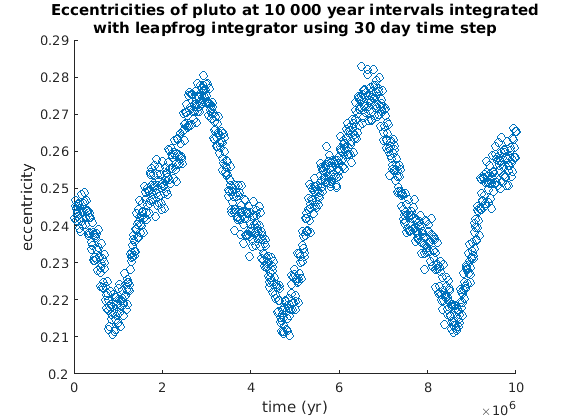
\includegraphics[width=\textwidth]{../plots/lf-longrun-eccentricity.png}
    \end{subfigure}
    \\
    \begin{subfigure}[b]{0.8\textwidth}
        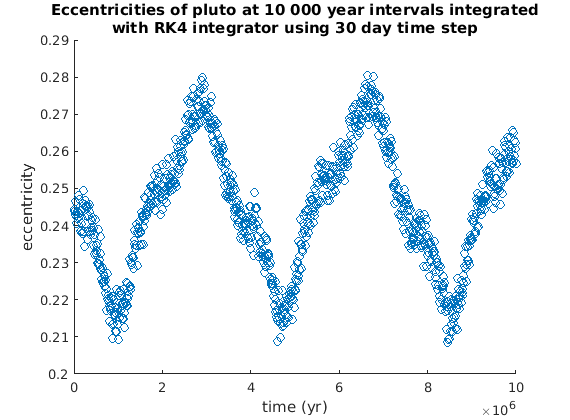
\includegraphics[width=\textwidth]{../plots/rk-longrun-eccentricity.png}
    \end{subfigure}
    \caption{Pluton radan eksentrisyyden vaihtelu $10^7$ vuoden aikana integroituna sekä leapfrog- että RK4-integraattorilla}\label{longrun-eccentricities}
\end{figure}

\begin{figure}[h!]
    \centering
    \begin{subfigure}[b]{0.8\textwidth}
        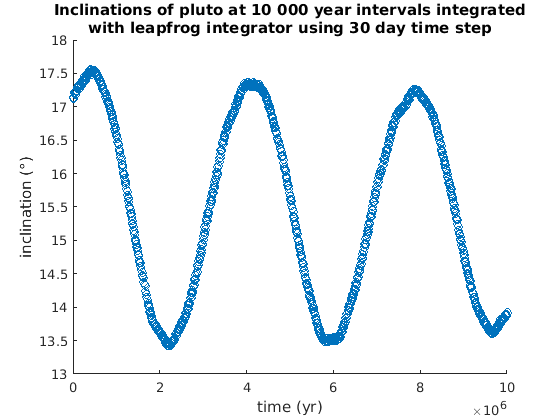
\includegraphics[width=\textwidth]{../plots/lf-longrun-inclination.png}
    \end{subfigure}
    \\
    \begin{subfigure}[b]{0.8\textwidth}
        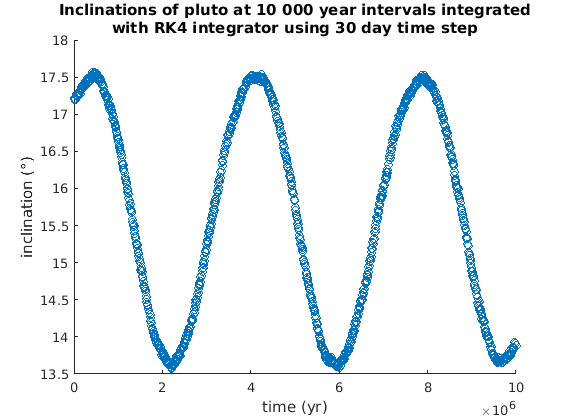
\includegraphics[width=\textwidth]{../plots/rk-longrun-inclination.png}
    \end{subfigure}
    \caption{Pluton radan inklinaation vaihtelu $10^7$ vuoden aikana integroituna sekä leapfrog- että RK4-integraattorilla}\label{longrun-inclinations}
\end{figure}

\subsection{Nousevan solmun prekessio}
Pluton nousevan solmun prekessio kumpaakin integraattoria käyttäen on nähtävissä kuvassa \ref{longrun-Omegas}. Etsimällä ajanhetket, joita seuraavalla hetkellä nousevan solmun pituuden arvo on suurempi kuin edellisellä ajanhetkellä (eli on ylitetty 360\textdegree raja), saadaan yhteen kierrokseen kuluvaksi ajaksi 
3 700 000 vuotta, joka vastaa prekessionopeutta \mbox{$-9,7\times 10^{-5}$ \textdegree /yr}.


\begin{figure}[h!]
    \centering
    \begin{subfigure}[b]{0.8\textwidth}
        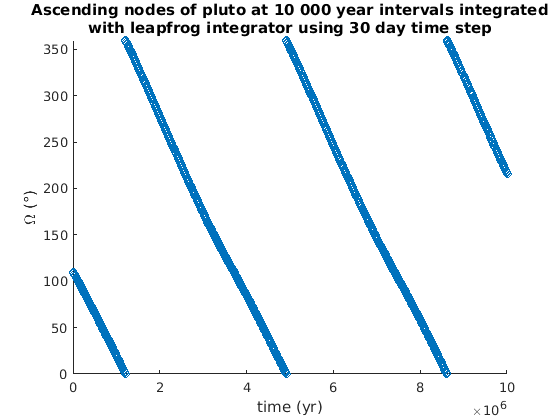
\includegraphics[width=\textwidth]{../plots/lf-longrun-Omega.png}
    \end{subfigure}
    \\
    \begin{subfigure}[b]{0.8\textwidth}
        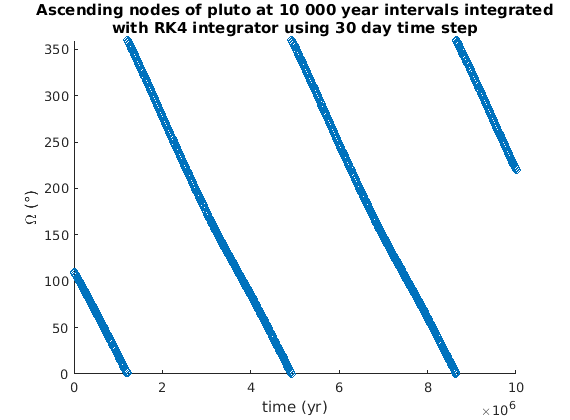
\includegraphics[width=\textwidth]{../plots/rk-longrun-Omega.png}
    \end{subfigure}
    \caption{Pluton radan nousevan solmun pituuden vaihtelu $10^7$ vuoden aikana integroituna sekä leapfrog- että RK4-integraattorilla}\label{longrun-Omegas}
\end{figure}

\subsection{Perhelin argumentti}
Kuten kuvasta \ref{longrun-omegas} nähdään, Pluton perihelin argumentti muuttuu periodisesti. Käytin Matlabin \texttt{cftool}ia sovittamaan dataan muotoa
$$a\sin{(bt+c)}+d$$
olevan käyrän, jolloin sain kummankin integraattorin datalla käyrän amplitudiksi $a$  noin 26\textdegree\ ja periodiksi $2\pi/b$ noin 3 800 000 vuotta.

\begin{figure}[h!]
    \centering
    \begin{subfigure}[b]{\textwidth}
        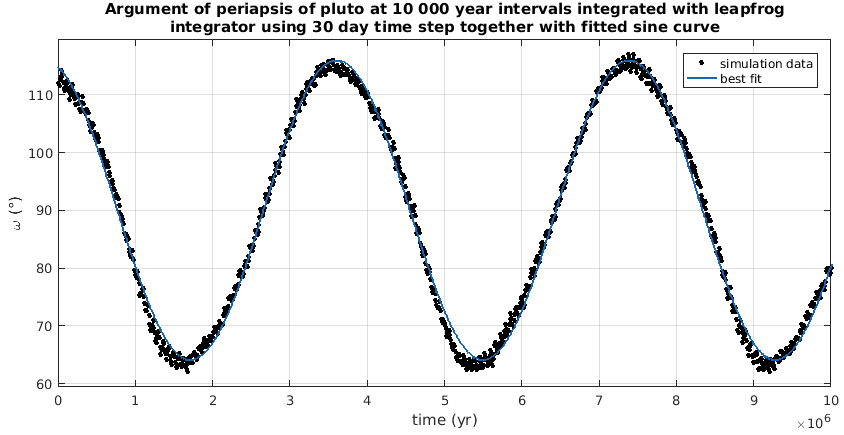
\includegraphics[width=\textwidth]{../plots/lf-longrun-omega-cut.png}
    \end{subfigure}
    \\
    \begin{subfigure}[b]{\textwidth}
        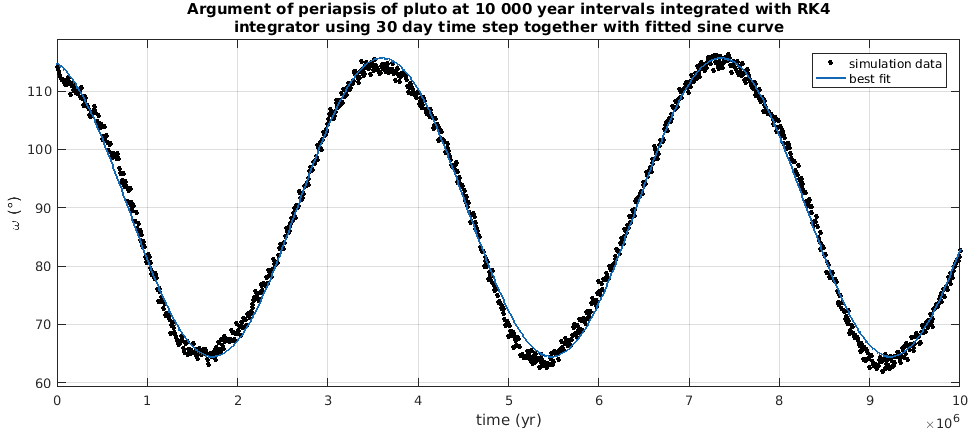
\includegraphics[width=\textwidth]{../plots/rk-longrun-omega-cut.png}
    \end{subfigure}
    \caption{Pluton radan perihelin argumentin vaihtelu $10^7$ vuoden aikana integroituna sekä leapfrog- että RK4-integraattorilla. Kummassakin kuvaajassa on lisäksi sinimuotoinen sovitus dataan yhtenäisellä viivalla esitettynä.}\label{longrun-omegas}
\end{figure}

\subsection{Pluto ja Neptunus}
Laskin lisäksi kummankin integraattorin datalla Pluton ja Neptunuksen dynamiikkaa kuvaavan parametrin
$$\phi_{32} = 3\lambda_P-2\lambda_N-\varpi.$$ Kummankin integraattorin tulosten mukaan oskillointi tapahtuu välillä 110--250\textdegree\ mikä vastaa amplitudia 70\textdegree\ ja keskiarvo periodin yli on noin 180\textdegree . On kuitenkin huomattavaa, että tutkittava väli ei ole periodin monikerta, jolloin keskiarvo ei täysin vastaa keskiarvoa yhden periodin yli. Paremmin oskillointia kuvaava luku saattaisi olla esimerkiksi ääriarvojen keskiarvo 180.

\begin{figure}[h!]
    \centering
    \begin{subfigure}[b]{0.8\textwidth}
        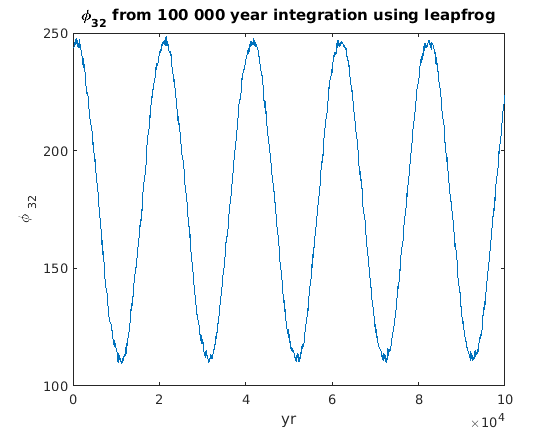
\includegraphics[width=\textwidth]{../plots/lf-shortrun-phi32.png}
    \end{subfigure}
    \\
    \begin{subfigure}[b]{0.8\textwidth}
        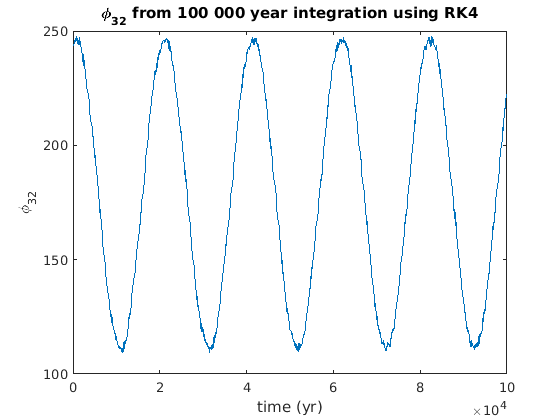
\includegraphics[width=\textwidth]{../plots/rk-shortrun-phi32.png}
    \end{subfigure}
    \caption{$\phi_{32}$:n vaihtelu $10 000$ vuoden aikana integroituna sekä leapfrog- että RK4-integraattorilla.}\label{shortrun-phis}
\end{figure}

\end{document}
